\chapter{APPENDICES}

\section*{Appendix A: Project Budget}
\addcontentsline{toc}{section}{Appendix A: Project Budget}
The project relies entirely on open-source software and publicly available climate datasets, keeping the overall budget minimal. Table \ref{tab:budget} summarizes the estimated costs.
\begin{table}[H]
\centering
\caption{Estimated Project Budget}
\label{tab:budget}
\normalsize
\renewcommand{\arraystretch}{1.2}
\begin{tabular}{|c|l|r|}
\hline
\textbf{S.N.} & \textbf{Item} & \textbf{Estimated Cost (NPR)} \\
\hline
1 & Google Colab Pro (3 months) & 8,000 \\
2 & Cloud storage / backup (Google Drive) & 500 \\
3 & Report printing and binding & 1,500 \\
4 & Stationery and miscellaneous & 500 \\
\hline
\multicolumn{2}{|r|}{\textbf{Total}} & \textbf{10,500} \\
\hline
\end{tabular}
\end{table}
\noindent
All datasets (ERA5, ORAS5, GODAS) are freely accessible through their respective portals for academic use. All software tools including Python, PyTorch, Xarray, and Scikit-learn are open-source with no licensing costs.

\section*{Appendix B: Project Timeline}
\addcontentsline{toc}{section}{Appendix B: Project Timeline}
\begin{figure}[H]
\centering
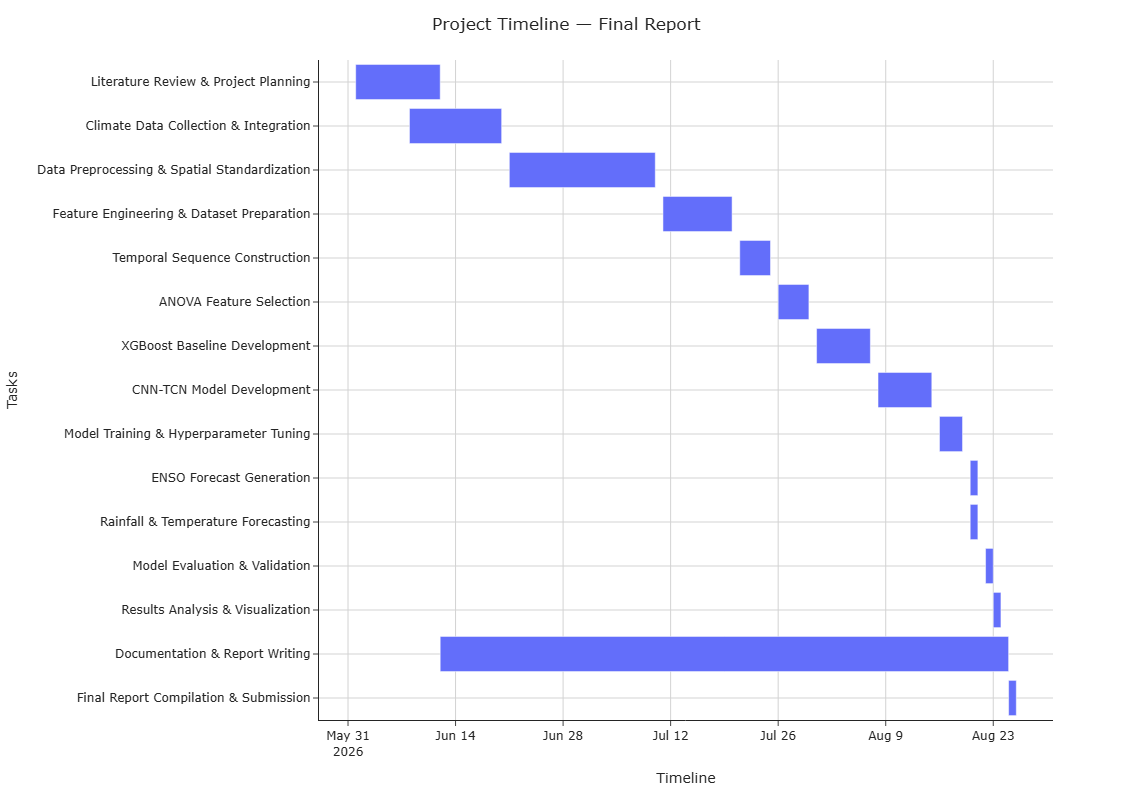
\includegraphics[width=\textwidth]{src/images/gantt_chart.png}
\caption{Project Timeline Gantt Chart}
\label{fig:gantt_chart}
\end{figure}

\newpage
\section*{Appendix C: Details of Dataset}
\addcontentsline{toc}{section}{Appendix C: Details of Dataset}

This appendix summarizes the datasets used for ENSO forecasting and South Asian regional climate impact assessment. Full acquisition and preprocessing details are given in Chapter~\ref{chap:implementation}; this appendix collects the source, coverage, resolution, and variable information for reference.

\subsection*{Dataset Overview}
Three datasets were used: two as model inputs (ERA5, ORAS5) and one as an independent validation reference (the NOAA Ni\~{n}o 3.4 index). All three cover the period 1980--2026, with a fixed 1980--2010 climatological baseline used for anomaly computation.

\begin{table}[H]
\centering
\caption{Summary of datasets used in the project}
\label{tab:dataset_summary}
\normalsize
\renewcommand{\arraystretch}{1.3}
\begin{tabularx}{\textwidth}{|>{\raggedright\arraybackslash}p{0.19\textwidth}|>{\raggedright\arraybackslash}p{0.16\textwidth}|>{\raggedright\arraybackslash}p{0.29\textwidth}|>{\raggedright\arraybackslash}X|}
\hline
\textbf{Dataset} & \textbf{Role} & \textbf{Source} & \textbf{Native Resolution} \\
\hline
ERA5 (Pacific) & Model input & Copernicus CDS & 0.25\degree, regridded to 2\degree \\
\hline
ERA5 (South Asia) & Model input & Copernicus CDS & 0.25\degree, regridded to 2\degree \\
\hline
ORAS5 & Model input & Copernicus CDS (ARCO Zarr) & Curvilinear NEMO grid \\
\hline
NOAA Ni\~{n}o 3.4 Index & Validation reference & NOAA Physical Sciences Laboratory & N/A (index only) \\
\hline
\end{tabularx}
\end{table}

\subsection*{ERA5 Reanalysis}
ERA5 is the fifth-generation atmospheric reanalysis produced by the European Centre for Medium-Range Weather Forecasts (ECMWF) and distributed through the Copernicus Climate Data Store (CDS) API. The monthly-mean product is used throughout this project. Two separate spatial extracts were pulled from the same underlying dataset.

\textbf{Pacific Ocean extract:}
\begin{itemize}
    \item \textbf{Purpose:} ENSO driver variables (SST, atmospheric fields).
    \item \textbf{Spatial domain:} 30\degree N to 30\degree S, 120\degree E to 280\degree E (80\degree W).
    \item \textbf{Resolution:} Regridded to 2\degree $\times$ 2\degree at request time via the CDS \texttt{grid} parameter.
    \item \textbf{Variables fetched:} Sea Surface Temperature (SST), 2-meter temperature, mean sea level pressure, zonal and meridional wind stress components, top-of-atmosphere thermal radiation, and the static land-sea mask (\texttt{lsm}).
\end{itemize}

\textbf{South Asia extract:}
\begin{itemize}
    \item \textbf{Purpose:} Regional climate impact assessment (precipitation and temperature response to ENSO).
    \item \textbf{Spatial domain:} 5\degree N to 35\degree N, 65\degree E to 100\degree E, covering the Indian subcontinent, Nepal, Bangladesh, and surrounding areas.
    \item \textbf{Resolution:} 2\degree $\times$ 2\degree, chosen to resolve regional topographic gradients (the Himalayas, the Western Ghats) that influence monsoon dynamics while remaining computationally tractable.
    \item \textbf{Variables fetched:} Precipitation, 2-meter temperature.
\end{itemize}

\subsection*{ORAS5 Ocean Reanalysis}
ORAS5 (Ocean ReAnalysis System 5) is ECMWF's operational ocean reanalysis, providing subsurface ocean variables not available from atmospheric reanalyses. It was accessed via its Analysis-Ready, Cloud-Optimized (ARCO) Zarr store rather than a direct CDS API request.
\begin{itemize}
    \item \textbf{Purpose:} Subsurface ocean memory predictors, principally Ocean Heat Content.
    \item \textbf{Native grid:} Curvilinear NEMO ocean model grid (not a regular latitude-longitude grid).
    \item \textbf{Regridding:} Interpolated to the same 2\degree $\times$ 2\degree regular grid as the ERA5 Pacific extract, using \texttt{xarray}'s \texttt{interp} method with bilinear interpolation.
    \item \textbf{Key variables:} Upper-300m Ocean Heat Content (\texttt{sohtc300}), sea surface height (\texttt{sossheig}), and 20\degree C isotherm depth (\texttt{so20chgt}), used across both feature-selection methodologies.
\end{itemize}

\subsection*{NOAA Ni\~{n}o 3.4 Index}
The official Ni\~{n}o 3.4 index, published by the NOAA Physical Sciences Laboratory, was not used as a model input. It served exclusively as an independent reference to validate the correctness of the computed Ni\~{n}o 3.4 index (area-averaged SST anomaly over 5\degree S--5\degree N, 170\degree W--120\degree W, against the 1980--2010 baseline). The computed and official indices achieved a Pearson correlation coefficient exceeding 0.95, confirming that the spatial subsetting, regridding, missing-value interpolation, and anomaly computation described in Chapter~\ref{chap:implementation} were implemented correctly.

\subsection*{Temporal Coverage and Splits}
All datasets span 1980--2026 at monthly resolution. After constructing 12-month sliding-window sequences (Section~\ref{sec:tensor-construction}), 542 valid samples remained, split strictly chronologically to prevent data leakage:

\begin{table}[H]
\centering
\caption{Chronological data split used across all models}
\label{tab:dataset_split}
\normalsize
\renewcommand{\arraystretch}{1.2}
\begin{tabular}{|l|l|l|}
\hline
\textbf{Split} & \textbf{Period} & \textbf{Samples} \\
\hline
Train & $\leq$ 2018 & 457 \\
\hline
Validation & 2019--2022 & 48 \\
\hline
Test & 2023--2026 & 40 \\
\hline
\end{tabular}
\end{table}

\subsection*{Final Feature Channels}
Of the variables listed above, four anomaly channels were retained in the spatio-temporal input tensor used by the CNN-TCN model and the two MIFS feature-selection methodologies:

\begin{table}[H]
\centering
\caption{Final input channels used in tensor construction}
\label{tab:dataset_channels}
\normalsize
\renewcommand{\arraystretch}{1.2}
\begin{tabular}{|l|l|l|}
\hline
\textbf{Channel} & \textbf{Variable} & \textbf{Source} \\
\hline
\texttt{sst\_anom} & Sea Surface Temperature anomaly & ERA5 \\
\hline
\texttt{msl\_anom} & Mean Sea Level Pressure anomaly & ERA5 \\
\hline
\texttt{avg\_iews\_anom} & Zonal wind stress anomaly & ERA5 \\
\hline
\texttt{sohtc300\_anom} & Upper-300m Ocean Heat Content anomaly & ORAS5 \\
\hline
\end{tabular}
\end{table}

\subsection*{Access and Licensing}
ERA5 and ORAS5 are both distributed by the Copernicus Climate Change Service (C3S) under the Copernicus license, which permits free use, modification, and redistribution with attribution. Access requires a (free) CDS account and API key. The NOAA Ni\~{n}o 3.4 index is publicly available from the NOAA Physical Sciences Laboratory website with no registration required.